\documentclass[conference]{IEEEtran}
\IEEEoverridecommandlockouts
% Based on IEEE-conference-template-062824

\usepackage{cite}
\usepackage{amsmath,amssymb,amsfonts}
\usepackage{algorithmic}
\usepackage{graphicx}
\usepackage{textcomp}
\usepackage{xcolor}
\usepackage{array}
\setlength{\dbltextfloatsep}{9pt plus 2pt minus 2pt}
\setlength{\textfloatsep}{7pt plus 2pt minus 2pt}
\setlength{\dblfloatsep}{6pt plus 2pt minus 2pt}
\setlength{\abovedisplayskip}{4pt plus 1pt minus 2pt}
\setlength{\belowdisplayskip}{4pt plus 1pt minus 2pt}
\def\BibTeX{{\rm B\kern-.05em{\sc i\kern-.025em b}\kern-.08em
    T\kern-.1667em\lower.7ex\hbox{E}\kern-.125emX}}

\begin{document}

\title{Tightening Deterministic Geometric Robustness Certification via
       Residual Factorized Networks and Linear Relaxation Bound Propagation}

\author{\IEEEauthorblockN{Sankalp Brahmapurkar}
\IEEEauthorblockA{\textit{Dept.\ of Information Technology}\\
Enrollment No.: IIT2023502}
\and
\IEEEauthorblockN{Parth Agrawal}
\IEEEauthorblockA{\textit{Dept.\ of Information Technology}\\
Enrollment No.: IIT2023506}
\and
\IEEEauthorblockN{Kunal}
\IEEEauthorblockA{\textit{Dept.\ of Information Technology}\\
Enrollment No.: IIT2023501}
}

\maketitle

\begin{abstract}
Deep neural networks remain vulnerable to continuous spatial transformations
such as image rotations, translations, and shear, which produce strongly
non-convex pixel perturbations.
Although Certified Geometric Training (CGT) paired with the Fast Geometric
Verifier (FGV) enabled deterministic training and certification under
geometric threat models~\cite{b3}, its reliance on plain Interval Bound
Propagation (IBP) and shallow three-layer convolutional architectures limits
bound tightness and clean generalization.
This work extends CGT across verification, optimization, and backbone design.
First, an adaptive Branch-and-Bound (BaB) verifier is introduced that replaces
box checks with specification-margin linear relaxations via CROWN-IBP and
incorporates concrete counterexample pre-falsification with multi-GPU sharding.
Second, a differentiable CROWN-IBP log-sum-exp margin loss is adopted during
training alongside compact residual backbones---a shallow Residual CNN for
MNIST and a Factorized Residual Network for CIFAR-10.
Evaluated on 1,000 CIFAR-10 test images under continuous rotation within
plus or minus 10 degrees, the Yang et al.\ reproduced baseline achieves
79.8\% clean accuracy and 62.6\% certified robustness.
Upgrading solely the network to the Factorized Residual Network under
unchanged IBP training raises certified robustness to 66.7\%.
Pairing the Factorized Residual Network with CROWN-IBP training and
verification reaches 82.1\% clean accuracy and 69.0\% certified robustness,
while cutting BaB node evaluations by 53.9\% relative to IBP-trained residual
models.
\end{abstract}

\begin{IEEEkeywords}
certified robustness, geometric transformations, interval bound propagation,
CROWN-IBP, residual networks, branch-and-bound
\end{IEEEkeywords}

%==========================================================================
\section{Introduction and Related Work}
%==========================================================================

\subsection{Motivation and Problem Scope}
Deep classifiers used in safety-critical perception systems encounter natural
geometric distortions including camera roll, translation, scaling, and shear.
Following the discovery of adversarial examples~\cite{b1}, empirical defenses
such as PGD adversarial training~\cite{b2} improved resilience but offer no
mathematical guarantee across continuous transformation sets.
Deterministic verification is therefore required to prove prediction invariance
for every parameter inside a target domain.

Unlike additive $\ell_p$ perturbations with independent pixel boxes, continuous
spatial warps couple adjacent pixels nonlinearly through bilinear
interpolation~\cite{b3},~\cite{b4}.
Yang et al.~\cite{b3} introduced CGT with the Fast Geometric Verifier (FGV)
to construct exact pixel interval over-approximations in parallel on GPUs,
enabling deterministic geometric training.
However, the base paper's CGT exhibits two bottlenecks: (1) pairing
axis-aligned IBP~\cite{b8} with shallow sequential CNNs restricts clean
accuracy and suffers loose bounds; (2) uniform static grid splitting wastes
compute evaluating fine sub-cells on inputs that could certify or fail early.

This work addresses these bottlenecks across four integrated contributions:
\vspace{-2pt}
\begin{enumerate}\setlength{\itemsep}{1pt}\setlength{\parskip}{0pt}
  \item The \texttt{certify.py} verifier is upgraded to evaluate
        specification-margin bounds via \texttt{IBP-C} and backward linear
        relaxation (\texttt{CROWN-IBP}) built on \texttt{auto\_LiRPA}~\cite{b11}
        inside an adaptive BaB search with concrete pre-falsification and
        multi-GPU sharding.
  \item Micro-batched differentiable \texttt{CROWN-IBP} margin training is
        implemented in \texttt{train.py} so backward graphs fit within 6\,GiB
        GPU VRAM.
  \item Residual skip-connected architectures~\cite{b14} are introduced into
        geometric verification---a 4-layer Residual CNN on MNIST~\cite{b15}
        and a Factorized Residual Network (\texttt{FactorizedResNet}) on
        CIFAR-10~\cite{b16}---with automatic checkpoint compatibility.
  \item Controlled ablations isolate architecture gains versus
        \texttt{CROWN-IBP} relaxation gains, measuring BaB node reduction and
        cross-verifier sensitivity.
\end{enumerate}
\vspace{-2pt}

\begin{figure*}[t]
\centering
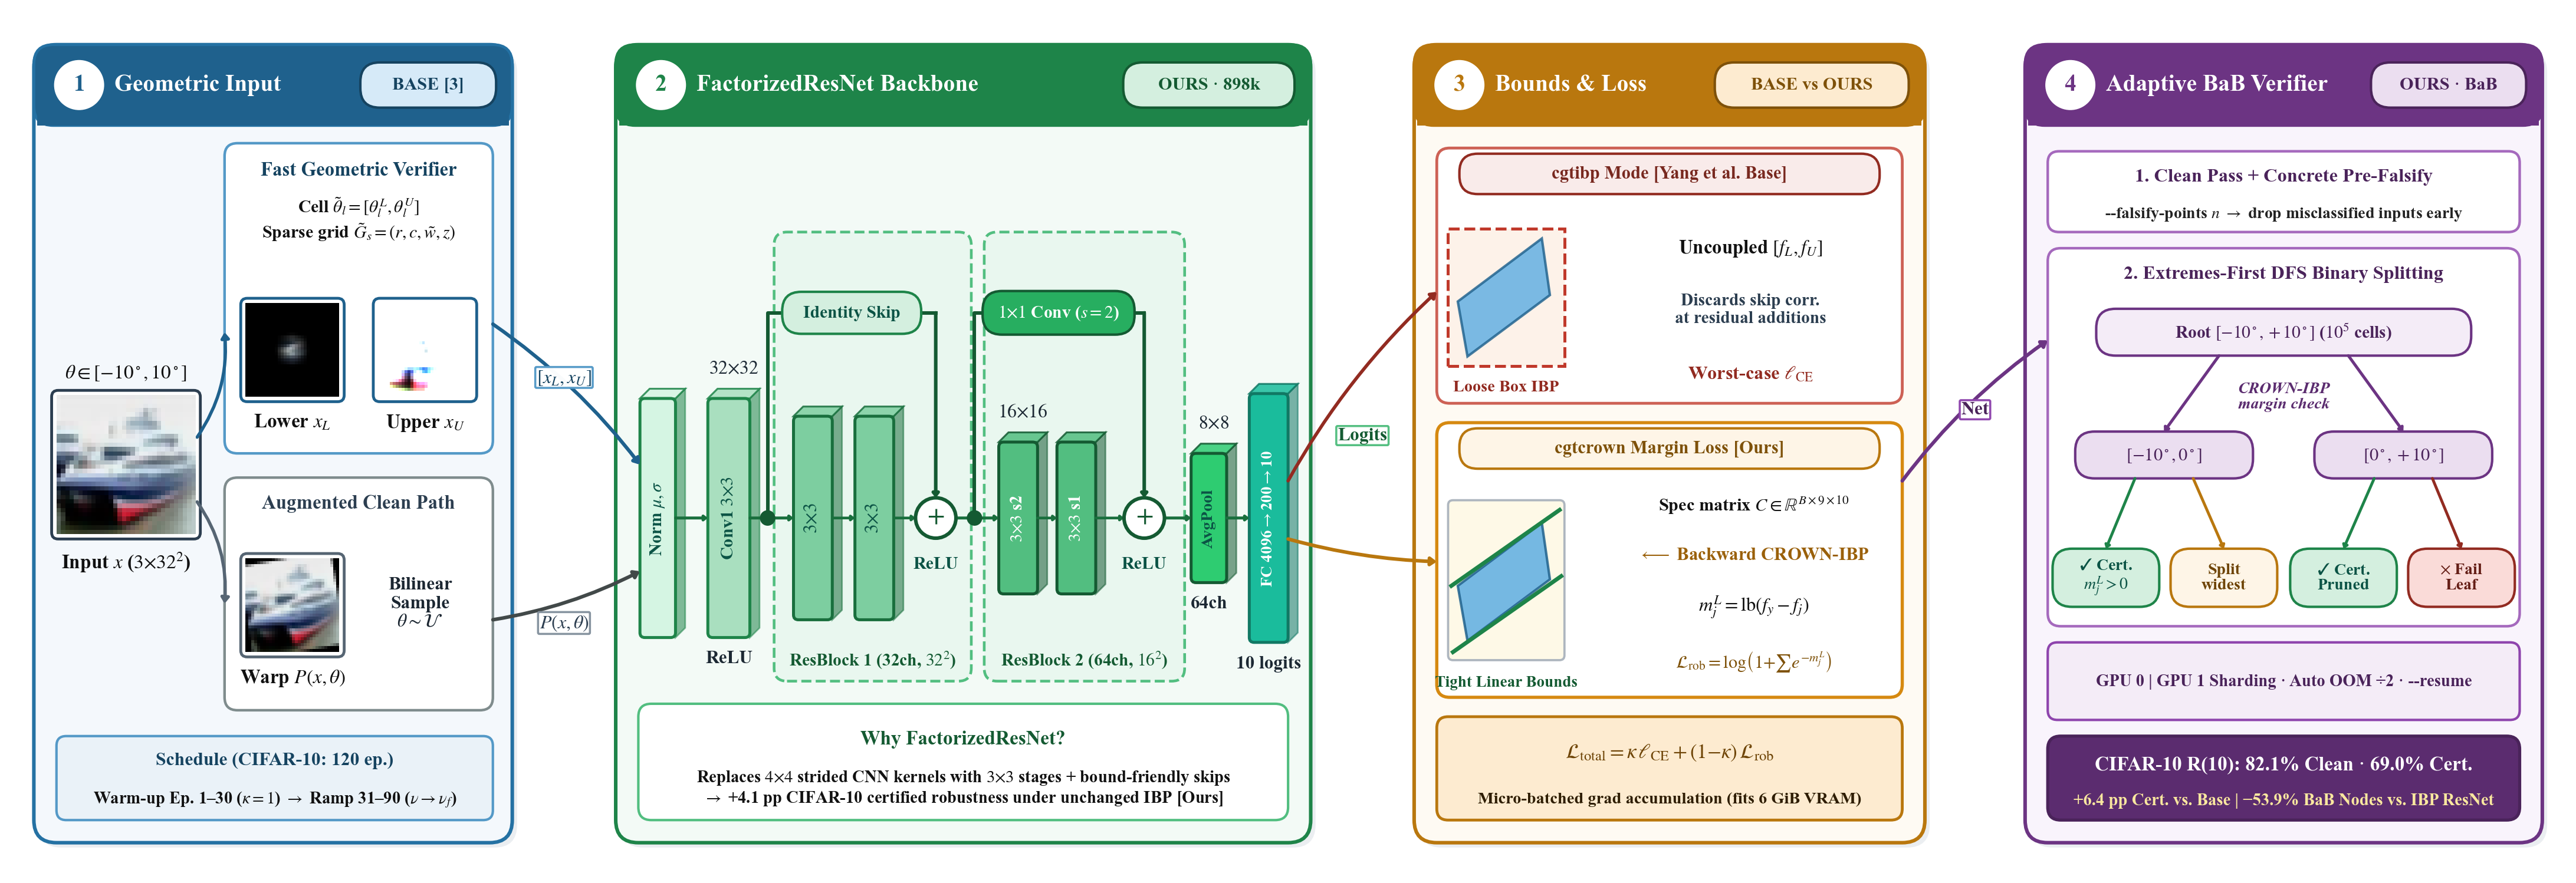
\includegraphics[width=0.98\textwidth]{methodology_diagram.png}
\caption{End-to-end pipeline proposed in this work:
  (Stage~1) FGV constructs pixel interval bounds $[x_L, x_U]$ from the
  Yang et al.\ geometric over-approximation scheme~\cite{b3};
  (Stage~2) bounds and augmented images are fed through the proposed
  \texttt{FactorizedResNet} backbone;
  (Stage~3) two training modes are compared---the Yang et al.\ \texttt{cgtibp}
  IBP loss and the \texttt{cgtcrown} CROWN-IBP margin loss proposed here;
  (Stage~4) an adaptive BaB certifier proposed in this work accelerates
  sound certification via pre-falsification, extremes-first DFS, and
  multi-GPU sharding.}
\label{fig:methodology}
\end{figure*}

\begin{table*}[t]
\caption{Component-Level Comparison: Yang et al.\ Base Paper~\cite{b3}
         versus Improvements Proposed in This Work}
\centering
\footnotesize
\setlength{\tabcolsep}{2.6pt}
\renewcommand{\arraystretch}{1.02}
\begin{tabular}{|l|>{\raggedright\arraybackslash}p{4.0cm}|>{\raggedright\arraybackslash}p{5.8cm}|>{\raggedright\arraybackslash}p{4.8cm}|}
\hline
\textbf{Dimension} &
\textbf{Yang et al.\ Base Paper~\cite{b3}} &
\textbf{This Work (Proposed Extension)} &
\textbf{Observed Improvement} \\
\hline
Network Backbone &
3-layer sequential CNN
(CIFAR-10: 666k params; MNIST: 663k params) &
Residual CNN (MNIST: 665k) and
\texttt{FactorizedResNet}
(CIFAR-10: 898k; $3{\times}3$ blocks + $1{\times}1$/id skips) &
\textbf{+4.1\,pp} CIFAR-10 cert.\ rob.\ under pure IBP
(62.6\% $\to$ 66.7\%) \\
\hline
Bound Propagation &
Axis-aligned box IBP only;
uncoupled skip additions &
Backward linear relaxation
(\texttt{CROWN-IBP} via
\texttt{auto\_LiRPA}~\cite{b11})
+ control \texttt{IBP-C} &
\textbf{+2.3\,pp} cert.\ rob.,
\textbf{+1.5\,pp} clean acc.\
(66.7\% $\to$ 69.0\%) \\
\hline
Training Objective &
Scalar worst-case IBP CE loss
(ep.\ 120 total: 0.656;
ramp peak 0.713) &
Micro-batched differentiable
\texttt{CROWN-IBP} log-sum-exp
spec margin loss &
Caps onset spike (1.87 vs.\ 6.96);
\textbf{$-$46.5\%} total loss
vs.\ base (0.351 vs.\ 0.656) \\
\hline
Certification Search &
Static uniform/plain IBP
grid evaluation &
Adaptive extremes-first DFS BaB,
\texttt{--falsify-points},
multi-GPU sharding, OOM halving &
\textbf{$-$53.9\%} BaB nodes vs.\
IBP ResNet (141.1k vs.\ 305.9k;
$-$46.6\% vs.\ Base CNN) \\
\hline
CIFAR-10 $R(10)$ Net &
79.8\% clean / 62.6\% cert.\ (1k repro.);
80.5\% / 63.2\% (10k~\cite{b3}) &
\texttt{FactorizedResNet} +
\texttt{cgtcrown} +
\texttt{CROWN-IBP} BaB (1k test images) &
\textbf{82.1\% clean / 69.0\% cert.}
(+6.4\,pp vs.\ repro.,
+5.8\,pp vs.\ paper 10k) \\
\hline
\end{tabular}
\label{tab:base_vs_ours}
\end{table*}

\subsection{Related Work}

\subsubsection{Bound Propagation for Norm-Bounded Verification}
Gowal \textit{et al.}~\cite{b8} demonstrated that IBP scales provable
$\ell_\infty$ training linearly with depth, though pure box bounds suffer
interval blow-up without heavy regularization.
To tighten bounds across nonlinearities, CROWN~\cite{b9} propagated linear
surrogate planes backward, and CROWN-IBP~\cite{b10} combined fast forward
IBP pre-activation bounds with backward CROWN relaxations to stabilize
certified training.
Xu \textit{et al.}~\cite{b11} generalized linear relaxation bound propagation
to arbitrary computational graphs via \texttt{auto\_LiRPA}, allowing residual
additions and pooling layers to be bounded differentiably.

\subsubsection{Geometric Certification Defenses}
DeepG~\cite{b4} derived sound linear relaxations over geometric compositions
using sampling and LP optimization, while Semantify-NN~\cite{b5} prepended
semantic input layers for standard $\ell_p$ verifiers; both incurred minutes
of CPU latency per sample.
Randomized smoothing extensions~\cite{b6} and Transformation-Specific
Smoothing (TSS)~\cite{b7} scale to deeper models via transformation noise,
yet provide only probabilistic guarantees.
Yang et al.~\cite{b3} overcame verification latency via FGV, attaining
$60{\times}$--$42{,}623{\times}$ speedups over DeepG.
The present work builds directly on the Yang et al.\ FGV framework to study
residual architectures and linear bound propagation within it.

\subsubsection{Branch-and-Bound and Residual Backbones}
Recursive domain refinement via BaB~\cite{b12} underpins modern complete
verifiers such as $\beta$-CROWN~\cite{b13}, which integrates split constraints
into GPU bound propagation.
ResNets~\cite{b14} ease gradient flow via shortcut connections, making compact
residual modules well-suited for CIFAR-10~\cite{b16} when paired with
correlation-preserving \texttt{CROWN-IBP} propagation.

%==========================================================================
\section{Methodology and Methodology Diagram}
%==========================================================================

Fig.~\ref{fig:methodology} illustrates the complete training and
deterministic certification pipeline proposed in this work.
Table~\ref{tab:base_vs_ours} directly contrasts each architectural,
optimization, and verification upgrade against the Yang et al.\ baseline~\cite{b3}.

\subsection{Fast Geometric Verifier and Interval Pixel Bounds}
Let $x \in [0, 1]^{C \times H \times W}$ undergo a transformation
parameterized by $\theta \in [\theta_{\min}, \theta_{\max}]$.
On a local sub-interval
$\tilde{\theta}_l = [\underline{\theta}_l, \overline{\theta}_l]$,
pixel coordinates $(i, j)$ map to centered Cartesian grid
$(u, v) = (j - \frac{W-1}{2},\; \frac{H-1}{2} - i)$.
Under planar rotation $\varphi \in [\underline{\varphi}, \overline{\varphi}]$,
Yang et al.'s FGV~\cite{b3} computes inverse coordinate intervals
monotonically across sub-quadrants as in~\eqref{eq:fgv_rot}:
\vspace{-3pt}
\begin{equation}
\begin{pmatrix} \tilde{u}' \\ \tilde{v}' \end{pmatrix}
=
\begin{pmatrix} \cos \tilde{\varphi} & \sin \tilde{\varphi} \\
                -\sin \tilde{\varphi} & \cos \tilde{\varphi} \end{pmatrix}
\begin{pmatrix} u \\ v \end{pmatrix}.
\label{eq:fgv_rot}
\end{equation}
\vspace{-3pt}
Bilinear weights form interval tensor
$\tilde{G} = \max(0, 1 - |\tilde{V}' - V|) \odot \max(0, 1 - |\tilde{U}' - U|)$.
Over 99\% of entries vanish outside four nearest neighbors; FGV extracts
sparse indices $(r, c)$, weights $\tilde{w} = [\underline{w}, \overline{w}]$,
and per-pixel counts $z$ into $\tilde{G}_s = (r, c, \tilde{w}, z)$,
producing sound batch pixel bounds via parallel GPU segment summation~\eqref{eq:fgv_bounds}:
\vspace{-3pt}
\begin{equation}
\mbox{\small $x_L\!=\!\mathrm{seg\_sum}(\underline{w}{\odot}x_{[:,:,r,c]}),\;
x_U\!=\!\mathrm{seg\_sum}(\overline{w}{\odot}x_{[:,:,r,c]}).$}
\label{eq:fgv_bounds}
\end{equation}

\begin{figure*}[t]
\centering
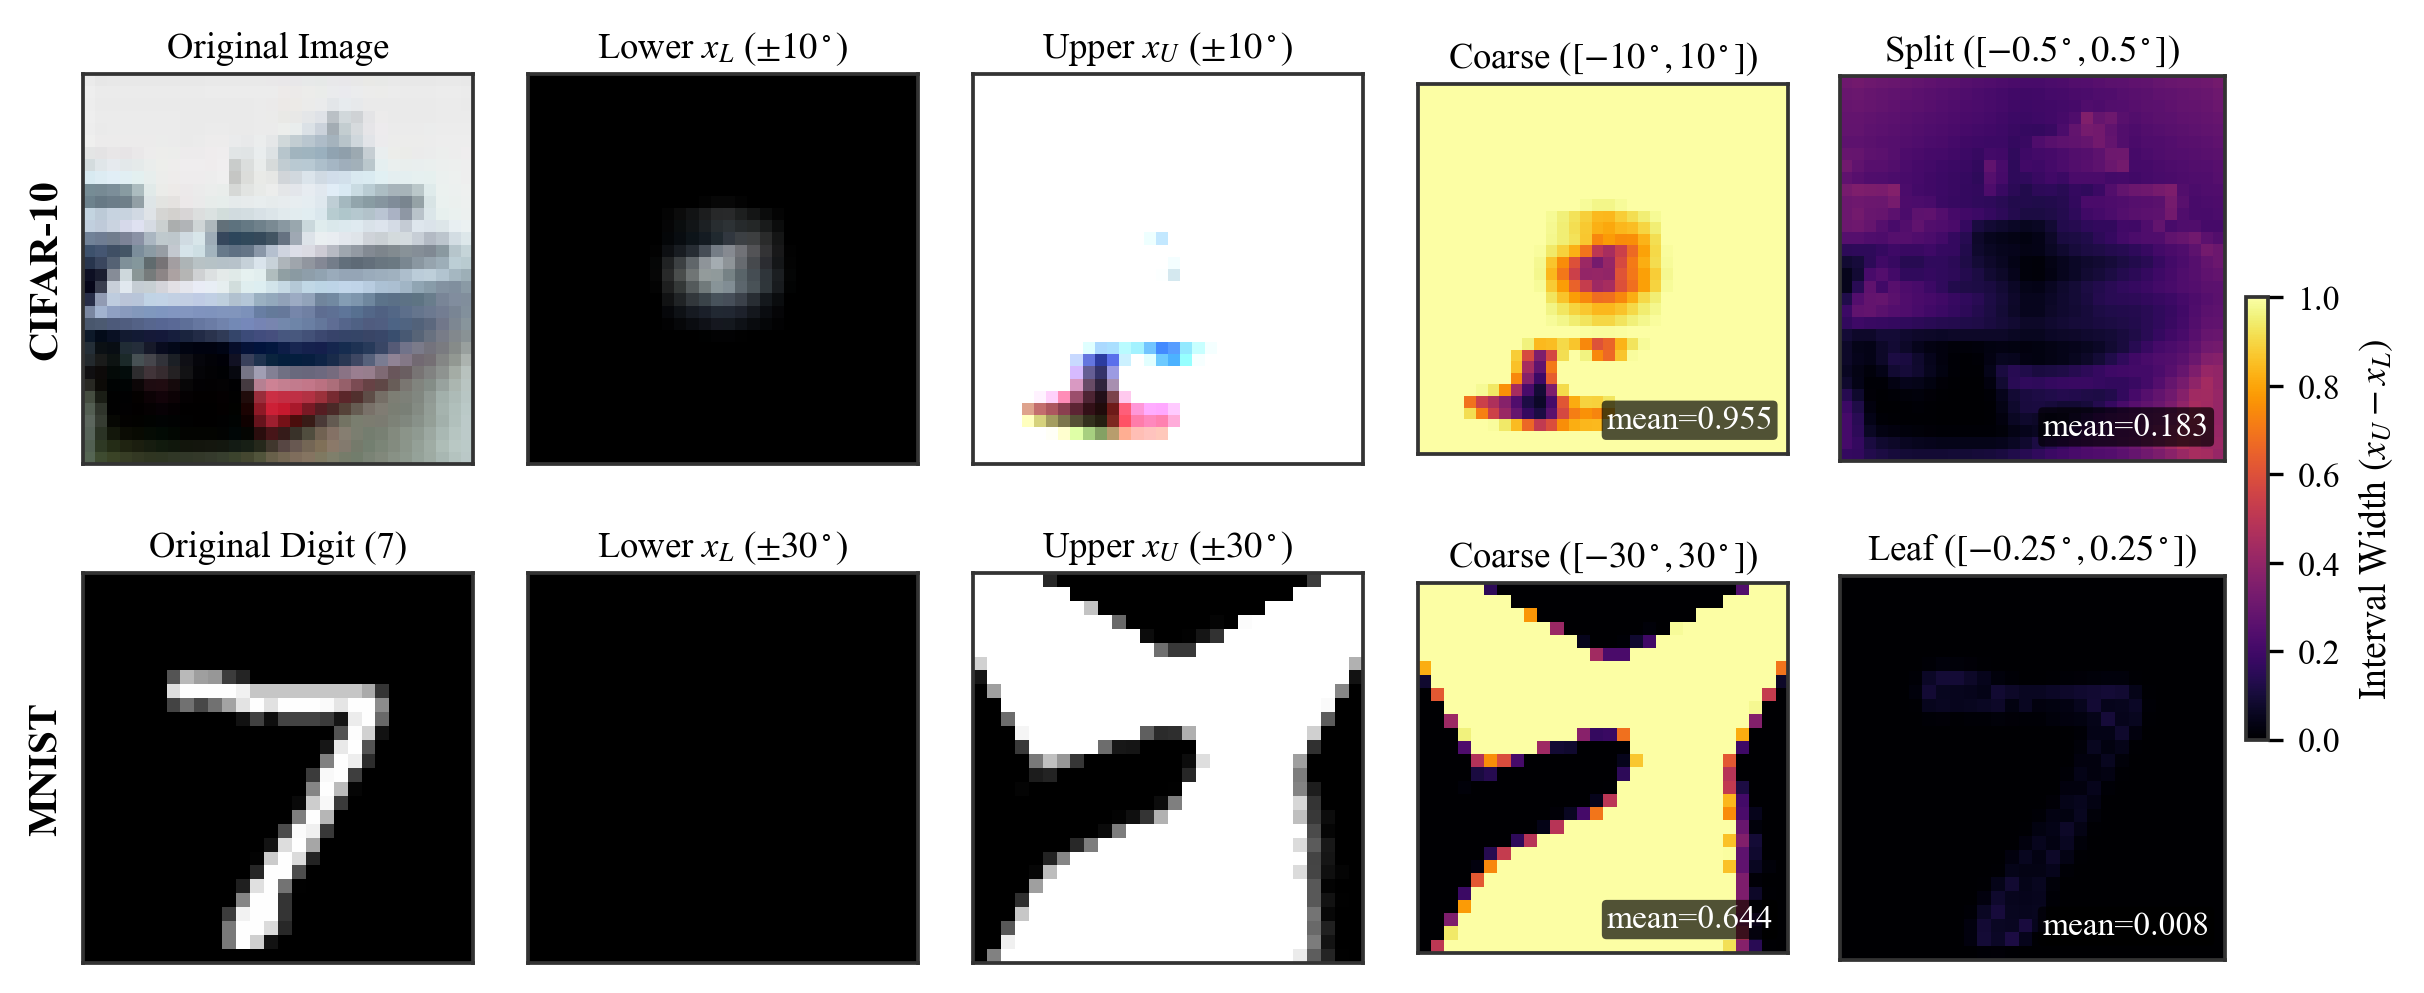
\includegraphics[width=0.62\textwidth]{fgv_interval_bounds.png}
\caption{FGV pixel bounds $x_L$, $x_U$, and interval width $(x_U - x_L)$
on CIFAR-10 (top row) and MNIST (bottom row) test samples computed using
the Yang et al.\ FGV implementation~\cite{b3}.
Coarse boxes yield wide bounds (mean width 0.955 on CIFAR-10; 0.644 on
MNIST), whereas sub-interval splitting tightens widths to 0.183 and 0.008
respectively.}
\label{fig:fgv_bounds}
\end{figure*}

\subsection{Residual CNN and Factorized Residual Network}
Because deep ResNets suffer severe IBP interval explosion across repeated
skip additions, this work designs shallow, bound-friendly residual networks
in \texttt{configs/}:

\subsubsection{MNIST Residual CNN (Experiment 3)}
After channel normalization ($\mu = 0.1307$, $\sigma = 0.3081$),
Layer~1 applies a $4{\times}4$ convolution ($1{\to}32$, $s{=}2$, $p{=}1$).
Layer~2 adds a $4{\times}4$ strided convolution ($32{\to}64$, $s{=}2$,
$p{=}1$) and a bias-free $1{\times}1$ projection shortcut ($32{\to}64$,
$s{=}2$) to align channels and $7{\times}7$ spatial shape, yielding
$\mathrm{ReLU}(\mathrm{conv}_2(x) + W_{1\times 1} x)$ before
$\mathrm{FC}(3136{\to}200{\to}10)$.

\subsubsection{CIFAR-10 FactorizedResNet (Experiment 4)}
For $3{\times}32{\times}32$ images, this work factorizes larger strided
kernels into consecutive $3{\times}3$ residual stages:
\vspace{-3pt}
\begin{itemize}\setlength{\itemsep}{1pt}\setlength{\parskip}{0pt}
  \item \textbf{Stem (\texttt{Conv1}):} Normalization followed by $3{\times}3$
        conv ($3{\to}32$, $s{=}1$, $p{=}1$) and ReLU.
  \item \textbf{ResBlock~1 ($32{\to}32$):} Two $3{\times}3$ convolutions
        ($s{=}1$, $p{=}1$) with identity shortcut
        $\mathrm{ReLU}(x + F_1(x))$.
  \item \textbf{ResBlock~2 ($32{\to}64$):} Downsampling $3{\times}3$ conv
        ($32{\to}64$, $s{=}2$) and $3{\times}3$ conv ($64{\to}64$, $s{=}1$)
        summed with a bias-free $1{\times}1$ shortcut ($32{\to}64$, $s{=}2$),
        producing $\mathrm{ReLU}(F_2(x) + S(x))$ at $16{\times}16$.
  \item \textbf{Head:} $2{\times}2$ average pooling outputs $64{\times}8{\times}8
        = 4096$ features into
        $\mathrm{FC}(4096{\to}200) \to \mathrm{ReLU} \to \mathrm{FC}(200{\to}10)$.
\end{itemize}
\vspace{-2pt}
Both architectures include \texttt{use\_residual} key auto-detection in
\texttt{certify.py} so Yang et al.'s sequential checkpoints and the
residual checkpoints proposed here load transparently.

\begin{table}[t]
\caption{Network Architectures and Parameter Counts}
\centering
\footnotesize
\setlength{\tabcolsep}{1.8pt}
\renewcommand{\arraystretch}{1.02}
\begin{tabular}{|l|>{\raggedright\arraybackslash}p{3.95cm}|r|}
\hline
\textbf{Model} & \textbf{Layer Configuration} & \textbf{Params} \\
\hline
MNIST Base~\cite{b3} &
  Conv(32,4,2)--Conv(64,4,2)--FC(200,10) & 662,786 \\
\hline
MNIST ResNet (Ours) &
  Conv(32,4,2)--Res(64,4,2 + 1$\times$1 s=2)--FC(200,10) & 664,834 \\
\hline
CIFAR Base~\cite{b3} &
  Conv(32,3,1)--Conv(32,4,2)--Conv(64,4,2)--FC(150,10) & 666,204 \\
\hline
\texttt{FactorizedResNet} (Ours) &
  Conv(32)--Res1(32)--Res2(64+1$\times$1)--AvgPool--FC(200,10) & 898,274 \\
\hline
\end{tabular}
\label{tab:architectures}
\end{table}

\begin{table}[t]
\caption{Training Schedules and Certification Granularity}
\centering
\footnotesize
\setlength{\tabcolsep}{2.4pt}
\renewcommand{\arraystretch}{1.02}
\begin{tabular}{|l|c|c|c|c|c|}
\hline
\textbf{Dataset} & \textbf{Ep.} & \textbf{BS} &
\textbf{Warm / Ramp} & \textbf{LR Drop} & \textbf{Cert.\ Cells} \\
\hline
MNIST (C0) & 100 & 256 & 15 / 50 ep. & Ep.\ 80 & 240 ($0.25^\circ$) \\
\hline
CIFAR-10 (C0) & 120 & 128 & 30 / 60 ep. & Ep.\ 100 & 100k ($0.0002^\circ$) \\
\hline
\end{tabular}
\label{tab:hyperparams}
\end{table}

\subsection{Differentiable CROWN-IBP Margin Training}
Yang et al.'s \texttt{cgtibp} training mode~\cite{b3} propagates uncoupled
interval bounds $[\underline{f}, \overline{f}]$, discarding linear correlations
between skip and main branches at each addition.
To preserve branch correlation during optimization, the \texttt{cgtcrown}
mode proposed in this work constructs specification matrix
$C \in \mathbb{R}^{B \times (K-1) \times K}$ with $C_{i,r,y_i} = 1$ and
$C_{i,r,j_r} = -1$ for each $j_r \neq y_i$, then runs backward
\texttt{CROWN-IBP}~\cite{b11} to obtain lower margin bounds~\eqref{eq:crown_margin}:
\vspace{-3pt}
\begin{equation}
m_j^L(x_L, x_U) =
  \mathrm{lb}_{\text{CROWN-IBP}}\!\big(f_y(x) - f_j(x)\big),\quad
  \forall\, j \neq y.
\label{eq:crown_margin}
\end{equation}
\vspace{-3pt}
A log-sum-exp robust margin surrogate is then minimized together with
clean augmented cross-entropy~\eqref{eq:total_loss}:
\vspace{-3pt}
\begin{equation}
\begin{aligned}
\mathcal{L}_{\mathrm{total}} &=
  \kappa\, \ell_{\mathrm{CE}}\!\big(f(P(x,\theta)),\, y\big) \\
  &\quad + (1 - \kappa)\log\!\bigl(1 + \textstyle\sum_{j \neq y} e^{-m_j^L(x_L, x_U)}\bigr).
\end{aligned}
\label{eq:total_loss}
\end{equation}
\vspace{-3pt}
After warm-up, $\kappa$ decays linearly from $1.0$ to $0.5$ while ball width
$\nu$ ramps from $0$ to $\nu_f$.
Gradient accumulation over \texttt{--robust-batch-size} chunks bounds peak
training memory.

\begin{figure*}[t]
\centering
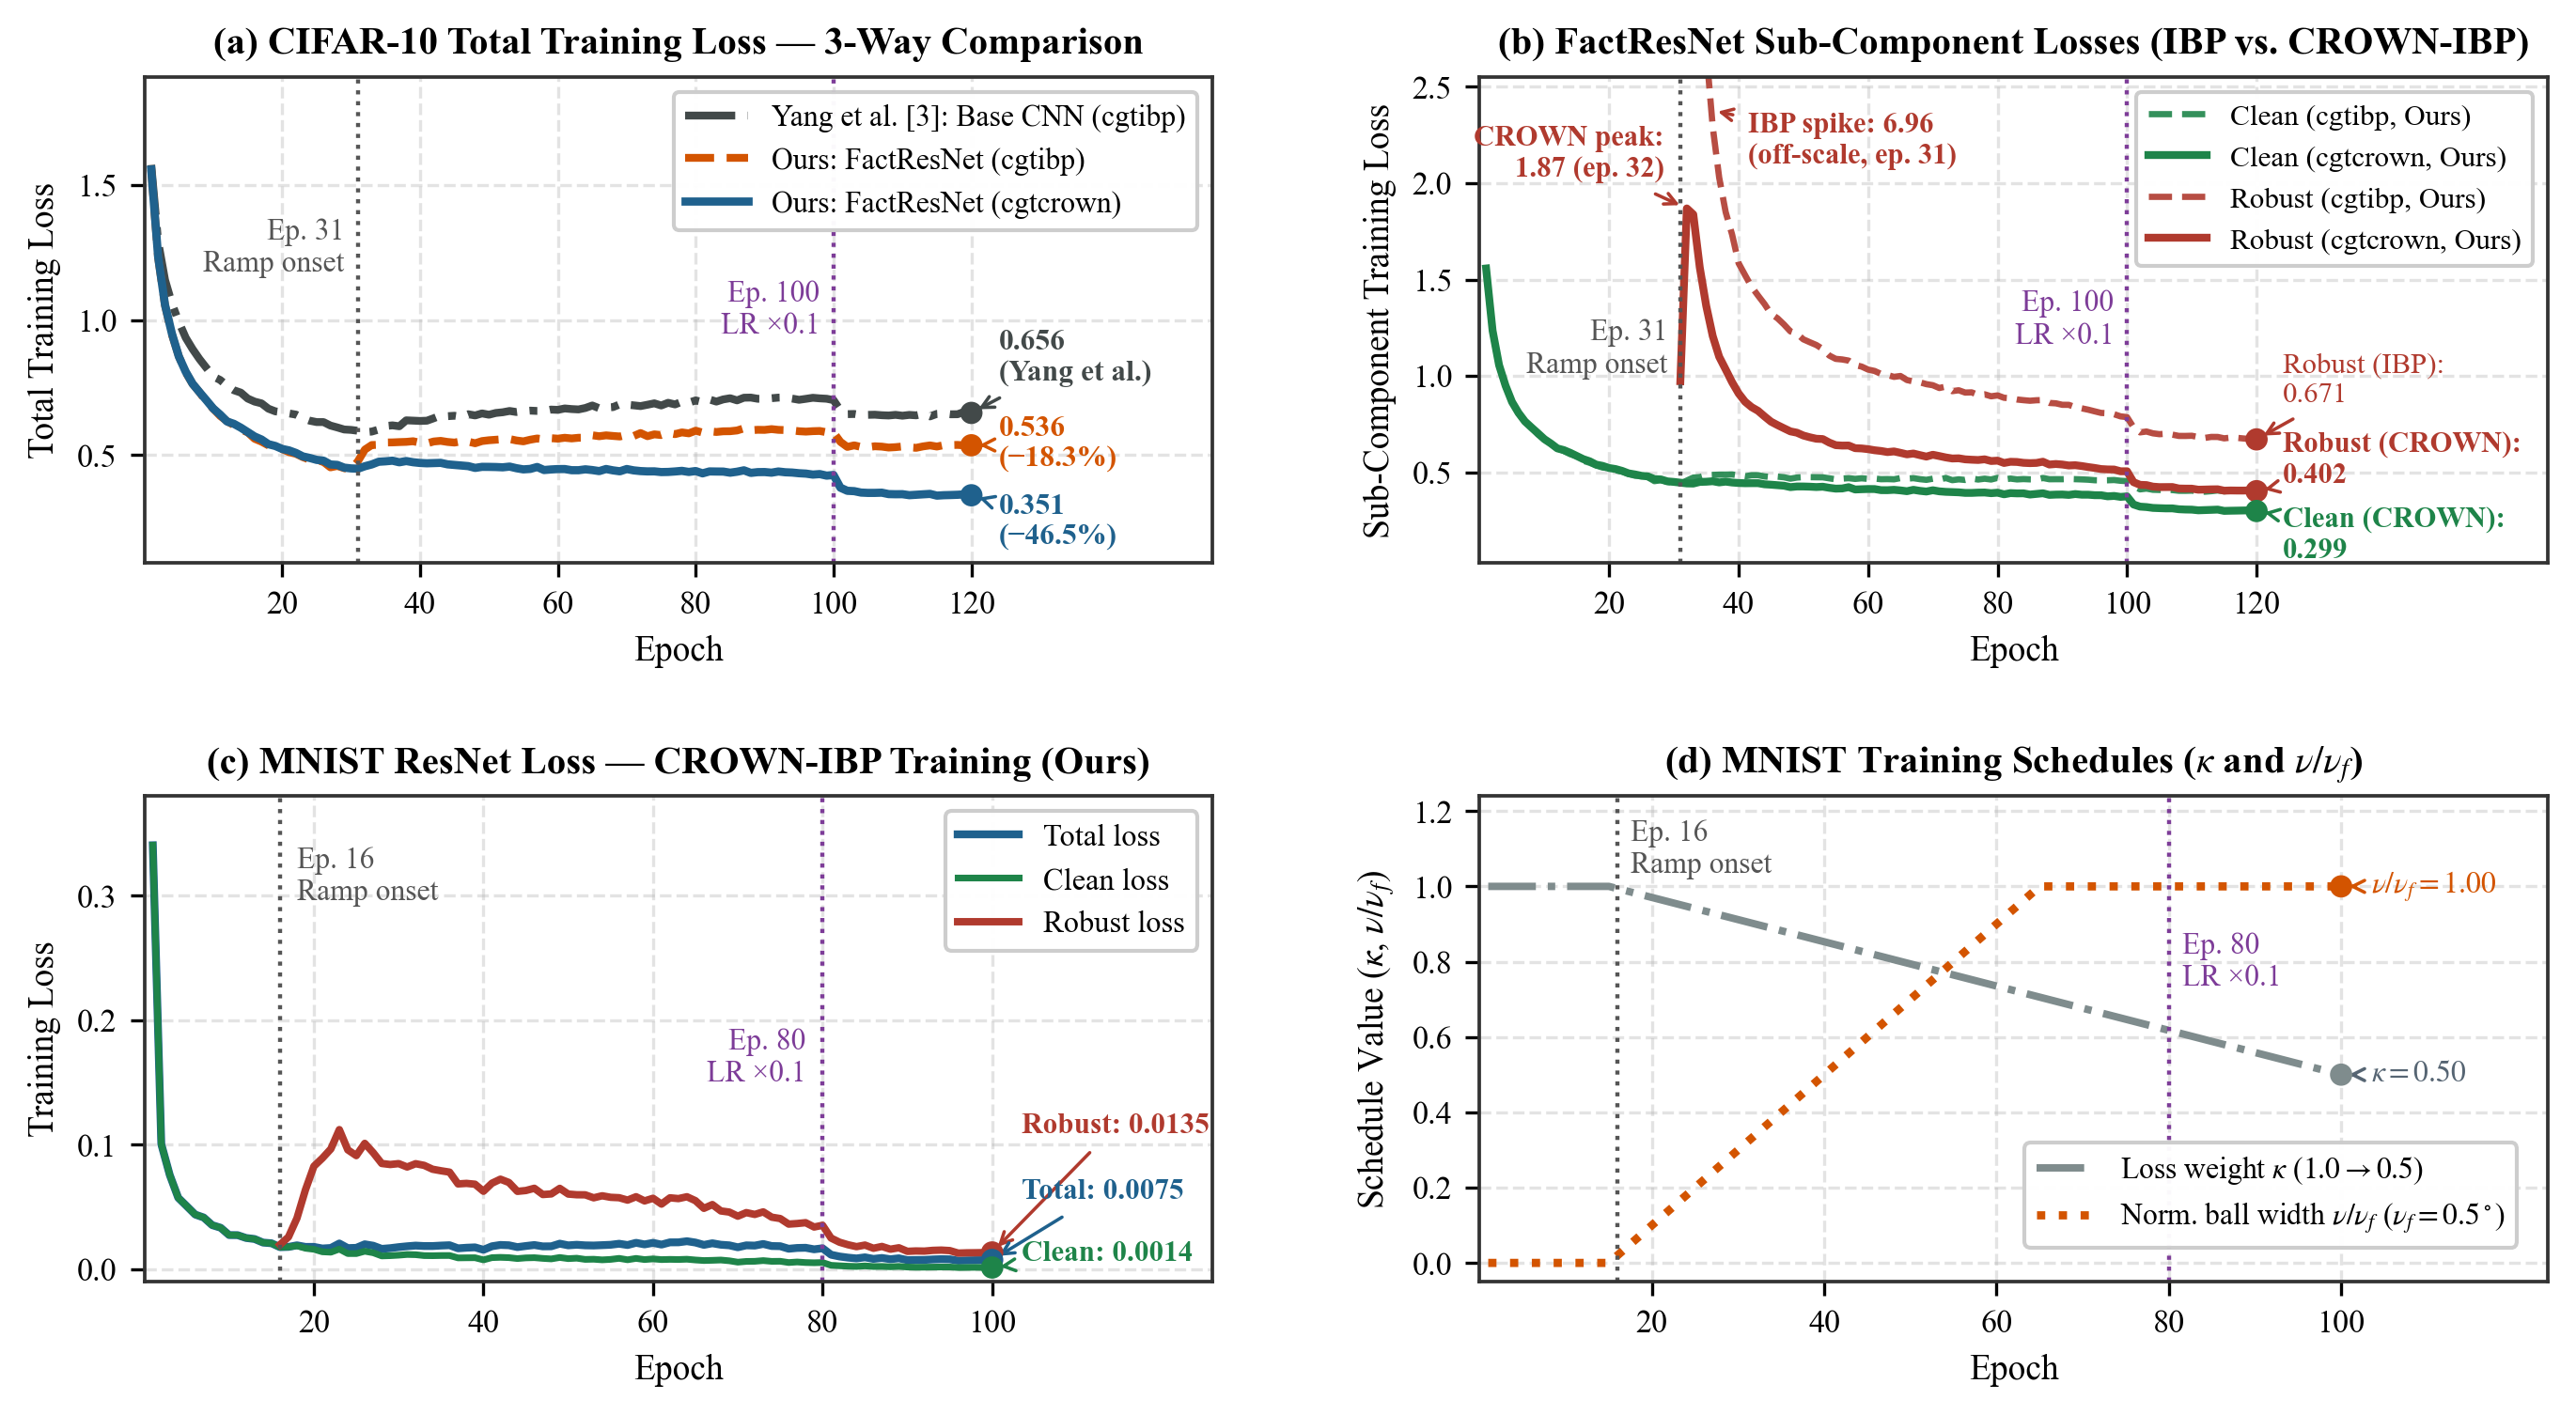
\includegraphics[width=0.86\textwidth]{training_loss_curves.png}
\caption{Training loss versus epochs from verified logs and local TensorBoard
  traces (120 epochs CIFAR-10; 100 epochs MNIST).
  \textbf{(a)}~Three-way CIFAR-10 total loss: the Yang et al.\ Base CNN
  (\texttt{cgtibp}~\cite{b3}) ends at 0.656; this work's
  \texttt{FactorizedResNet} under \texttt{cgtibp} reduces loss by 18.3\%
  to 0.536; \texttt{FactorizedResNet} under \texttt{cgtcrown} (this work)
  reduces loss by 46.5\% to 0.351.
  \textbf{(b)}~Sub-component clean and robust losses for the proposed
  \texttt{FactorizedResNet} under both training modes (Yang et al.'s
  \texttt{cgtibp} has only aggregate loss logged).
  \textbf{(c)}~Total, clean, and robust losses for the proposed MNIST
  Residual CNN under \texttt{cgtcrown}.
  \textbf{(d)}~Training schedule curves ($\kappa$ and $\nu/\nu_f$) for
  the proposed MNIST Residual CNN.}
\label{fig:loss_curves}
\end{figure*}

\begin{table*}[t]
\caption{MNIST Rotation ($[-30^\circ, +30^\circ]$) Verifier and
         Training Margin Ablation (100 Test Images, Batch Size 32)}
\centering
\footnotesize
\setlength{\tabcolsep}{4.8pt}
\renewcommand{\arraystretch}{1.04}
\begin{tabular}{|l|l|c|c|c|c|c|}
\hline
\textbf{Model Checkpoint} &
\textbf{Train Loss} &
\textbf{Verifier} &
\textbf{Clean Acc.} &
\textbf{Certified Rob.} &
\textbf{Cert.\ Time} &
\textbf{Peak VRAM} \\
\hline
Yang et al.\ Baseline~\cite{b3} & IBP Loss & \texttt{IBP}
  & 99.0\% (99/100) & 94.0\% & 10.68\,s & 33.57\,MB \\
Yang et al.\ Baseline~\cite{b3} & IBP Loss & \texttt{IBP-C}
  & 99.0\% (99/100) & 94.0\% & 4.87\,s & 33.57\,MB \\
Yang et al.\ Baseline~\cite{b3} & IBP Loss & \texttt{CROWN-IBP}
  & 99.0\% (99/100) & \textbf{96.0\%} & 33.97\,s & 79.05\,MB \\
\hline
Exp.~2 Seq.\ CNN (Ours) & CROWN-IBP Margin & \texttt{IBP}
  & 99.0\% (99/100) & 90.0\% & 8.11\,s & 33.57\,MB \\
Exp.~2 Seq.\ CNN (Ours) & CROWN-IBP Margin & \texttt{IBP-C}
  & 99.0\% (99/100) & 91.0\% & 8.29\,s & 33.57\,MB \\
Exp.~2 Seq.\ CNN (Ours) & CROWN-IBP Margin & \texttt{CROWN-IBP}
  & 99.0\% (99/100) & \textbf{96.0\%} & \textbf{24.67\,s} & 79.05\,MB \\
\hline
\end{tabular}
\label{tab:mnist_ablation}
\end{table*}

\subsection{Adaptive Branch-and-Bound Certification}
Uniformly verifying $100{,}000$ fine cells on CIFAR-10 is prohibitively
redundant for easy samples.
The BaB certifier proposed in this work accelerates sound certification in
three steps:
\vspace{-3pt}
\begin{enumerate}\setlength{\itemsep}{1pt}\setlength{\parskip}{0pt}
  \item \textbf{Clean Pass \& Pre-Falsification:} Clean-correct images are
        cached once; optional \texttt{--falsify-points} evaluates $n$ concrete
        angles and discards provably misclassified inputs upfront.
  \item \textbf{Coarse-to-Fine Evaluation:} Starting from the full
        transformation box, \texttt{certify.py} evaluates mini-batches via
        \texttt{IBP}, control \texttt{IBP-C}, or \texttt{CROWN-IBP}.
        Any sub-box satisfying $m_j^L > 0\;\forall\, j \neq y$
        immediately certifies its cell count.
  \item \textbf{Extremes-First DFS Splitting:} Remaining boxes bisect along
        their widest axis (\texttt{split\_node}), ordering outer angles first
        on the DFS stack to reject fragile images early, with multi-GPU
        sharding, checkpoint \texttt{--resume}, and automatic CUDA OOM batch
        halving.
\end{enumerate}
\vspace{-2pt}

%==========================================================================
\section{Experimental Settings}
%==========================================================================

\subsection{Datasets and Perturbation Threat Models}
Experiments use MNIST~\cite{b15} ($28{\times}28$ grayscale; 60k train, 10k
test, and 100-image slices for Experiments~1--2) under Config~0 rotation
$[-30^\circ, +30^\circ]$ ($w = 0.5^\circ$ training;
$w = 0.25^\circ$, 240 cells certification), and CIFAR-10~\cite{b16}
($32{\times}32$ RGB; 50k train with padding-4 random crop and horizontal
flip; 1,000 test images for Experiment~4) under Config~0 rotation
$[-10^\circ, +10^\circ]$ ($w = 0.001^\circ$ training;
$w = 0.0002^\circ$, 100k cells certification).

\subsection{Architectures, Schedules, and Hardware}
Tables~\ref{tab:architectures} and~\ref{tab:hyperparams} list exact model
layers, parameter counts, and training schedules.
All runs optimize with Adam ($\text{lr} = 10^{-3}$, gradient clip norm 8.0).
Local training ran on an NVIDIA GeForce RTX~3050 Laptop GPU (6.0\,GiB VRAM);
1,000-image CIFAR-10 certifications ran across two Kaggle GPUs
(\texttt{--num-gpus 2}, \texttt{eval\_batch\_size=1024}).

%==========================================================================
\section{Results and Ablation Studies}
%==========================================================================

\subsection{Interval Uncertainty and Training Loss Dynamics}
Fig.~\ref{fig:fgv_bounds} illustrates why recursive splitting is essential:
at full range, mean pixel width reaches $0.955$ on CIFAR-10 and $0.644$ on
MNIST, dropping sharply to $0.183$ and $0.008$ after domain refinement.

\begin{figure*}[t]
\centering
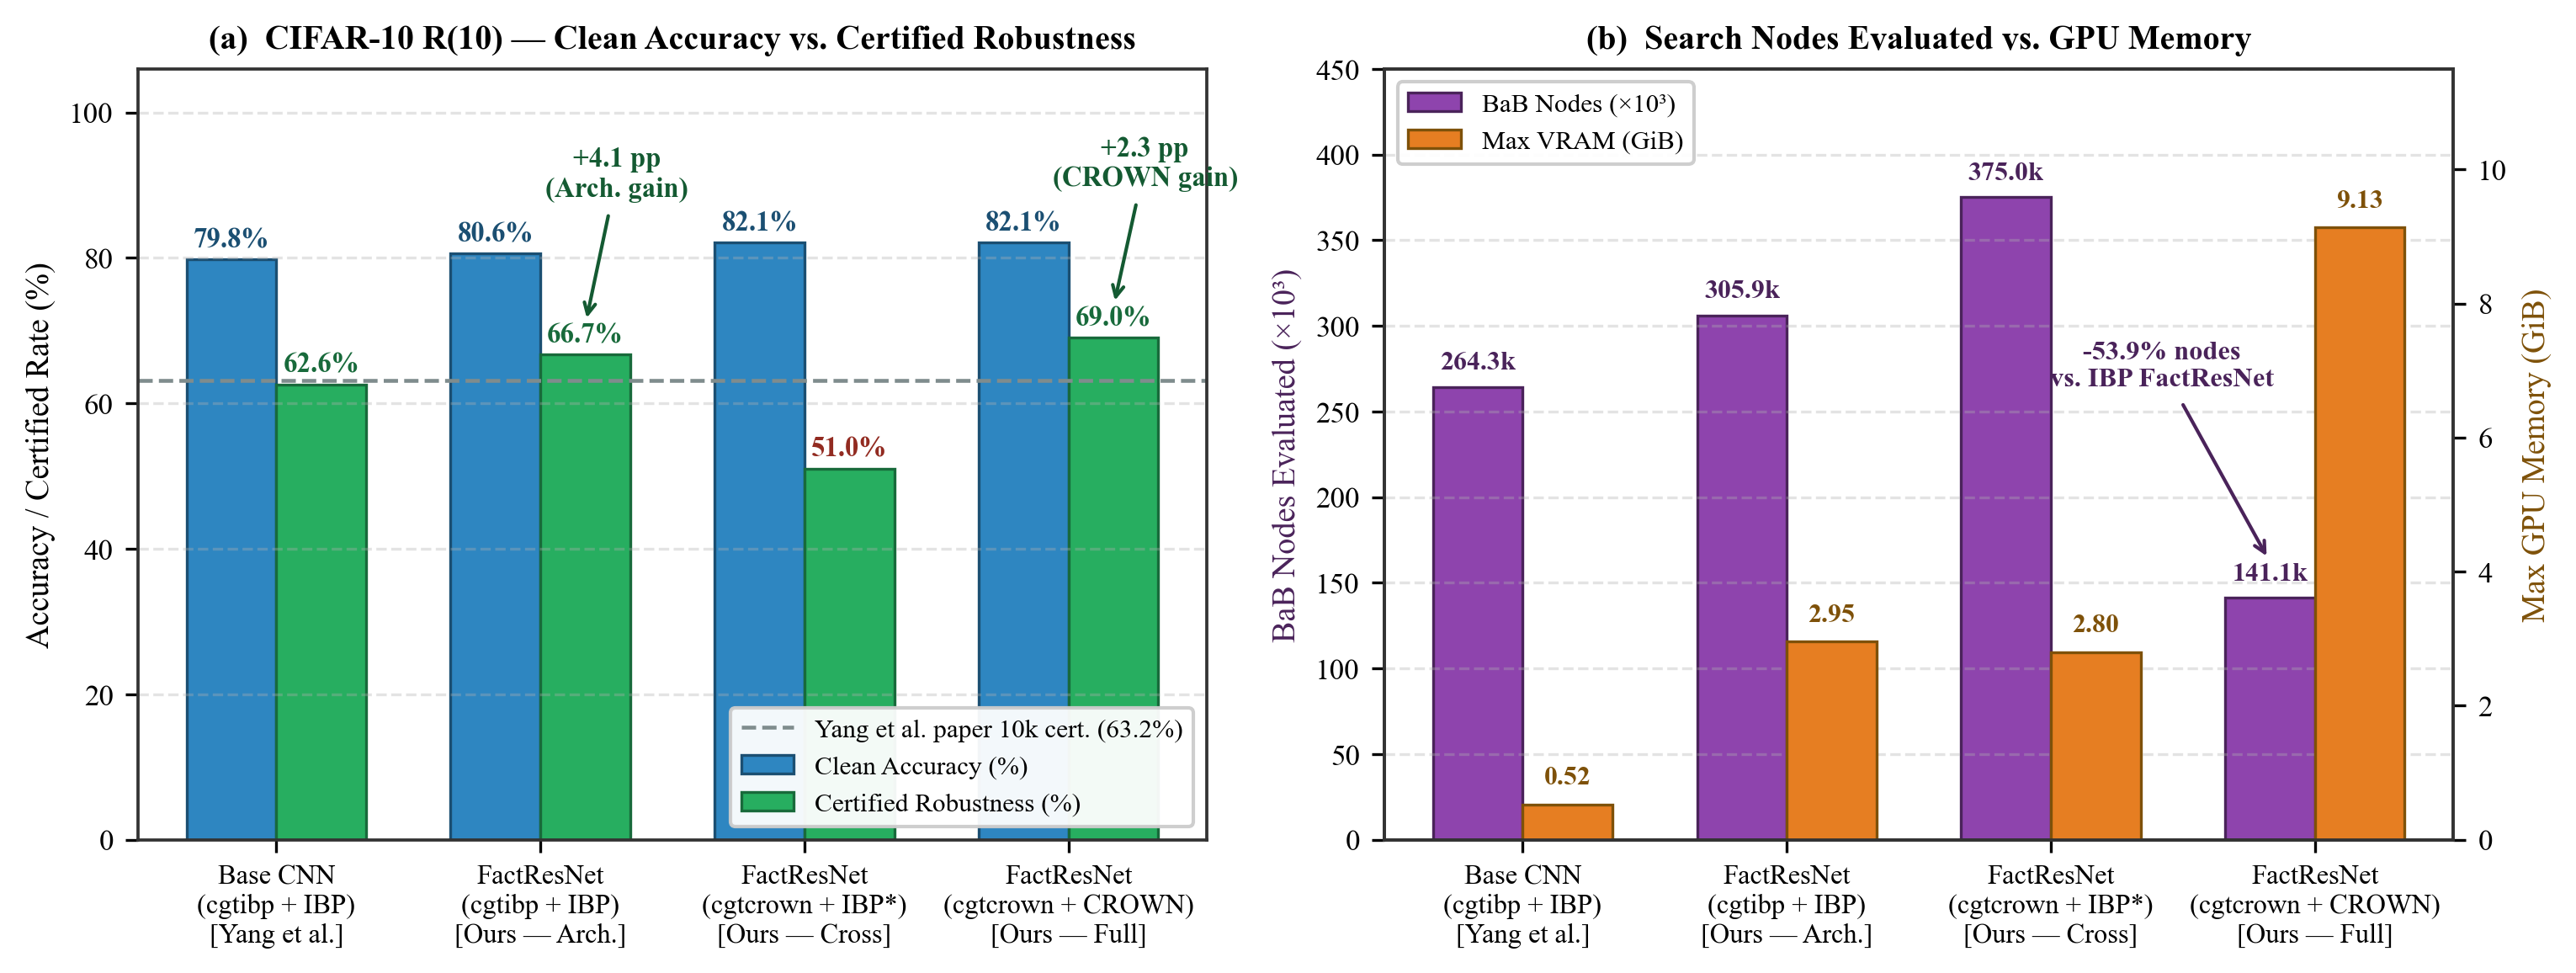
\includegraphics[width=0.94\textwidth]{cifar10_ablation_comparison.png}
\caption{Four-way CIFAR-10 Rotation $R(10)$ ablation across 1,000 test images.
  (a)~\texttt{FactorizedResNet} (this work) contributes
  $+4.1\,\text{pp}$ certified robustness over the Yang et al.\ baseline
  under fixed IBP settings; adding \texttt{CROWN-IBP} training and
  verification (this work) contributes a further $+2.3\,\text{pp}$
  robustness and $+1.5\,\text{pp}$ clean accuracy; mismatched
  verifier (\texttt{IBP*}) drops certified accuracy to 51.0\%.
  (b)~\texttt{CROWN-IBP} cuts BaB nodes by 53.9\% relative to the
  IBP-trained \texttt{FactorizedResNet} ($141.1\text{k}$ vs.\ $305.9\text{k}$).}
\label{fig:ablation}
\end{figure*}

\begin{table*}[t]
\caption{CIFAR-10 Rotation ($[-10^\circ, +10^\circ]$) Four-Way Ablation
         on 1,000 Test Images (2 GPUs, \texttt{eval\_batch\_size=1024})}
\centering
\footnotesize
\setlength{\tabcolsep}{2.6pt}
\renewcommand{\arraystretch}{1.06}
\begin{tabular}{|l|l|l|c|c|c|r|r|r|}
\hline
\textbf{Architecture} &
\textbf{Train} &
\textbf{Certify} &
\textbf{Clean Acc.} &
\textbf{Cert.\ Rob.} &
\textbf{$\Delta$ vs.\ Base} &
\textbf{BaB Nodes} &
\textbf{Cert.\ Time} &
\textbf{Max VRAM} \\
\hline
Paper Baseline (10k)~\cite{b3} &
  \texttt{cgtibp} & \texttt{IBP} &
  80.5\% & 63.2\% & N/A (10k imgs) & -- & -- & -- \\
\hline
Base 3-Layer CNN (Repro.)~\cite{b3} &
  \texttt{cgtibp} & \texttt{IBP} &
  79.8\% (798) & 62.6\% (626) & Ref. & 264,320 & 955.4\,s & 531.39\,MB \\
\texttt{FactorizedResNet} (Arch., Ours) &
  \texttt{cgtibp} & \texttt{IBP} &
  80.6\% (806) & 66.7\% (667) & +4.1\,pp & 305,920 & 1835.8\,s & 3024.31\,MB \\
\texttt{FactorizedResNet} (Cross, Ours) &
  \texttt{cgtcrown} & \texttt{IBP} &
  \textbf{82.1\%} (821) & 51.0\% (510) & $-$11.6\,pp & 375,000 & 5169.4\,s & 2868.99\,MB \\
\texttt{FactorizedResNet} (Full, Ours) &
  \texttt{cgtcrown} & \texttt{CROWN-IBP} &
  \textbf{82.1\%} (821) & \textbf{69.0\%} (690) & \textbf{+6.4\,pp} &
  \textbf{141,142} & 9270.8\,s & 9350.99\,MB \\
\hline
\end{tabular}
\label{tab:cifar_ablation}
\end{table*}

Fig.~\ref{fig:loss_curves} presents training loss trajectories from all
evaluated models.
On CIFAR-10 (Fig.~\ref{fig:loss_curves}(a)), this work's
\texttt{FactorizedResNet} already outperforms the Yang et al.\ 3-layer
baseline CNN during clean warm-up ($0.4459$--$0.4501$ vs.\ $0.5928$ at
epoch 30).
During the perturbation ramp (epochs 31--90, $\nu: 0 \to 0.001^\circ$,
$\kappa: 1.0 \to 0.5$), the Yang et al.\ base CNN's total loss rebounds
to a ramp peak of $0.7131$ (epoch 93) and finishes at $0.6558$
($28.5\,\text{min}$ on Kaggle).
Upgrading to \texttt{FactorizedResNet} under identical \texttt{cgtibp}
training (this work) reduces epoch-120 total loss by $18.3\%$ to $0.5358$
($97.1\,\text{min}$ local), whereas pairing \texttt{FactorizedResNet} with
linear relaxation (\texttt{cgtcrown}, this work) maintains steady descent
across the ramp and converges to $0.3505$---a $46.5\%$ reduction over the
Yang et al.\ base paper and $34.6\%$ below the IBP-trained \texttt{FactorizedResNet}
($364.6\,\text{min}$ total).

The sub-component view (Fig.~\ref{fig:loss_curves}(b)) shows that
\texttt{cgtibp} training triggers a $6.963$ robust CE spike at epoch~31
onset, while \texttt{cgtcrown} caps the transient peak at $1.869$
(epoch 32) and finishes lower in both clean ($0.2991$ vs.\ $0.4010$) and
robust loss ($0.4020$ vs.\ $0.6707$).
On MNIST (Figs.~\ref{fig:loss_curves}(c)--(d)), the Residual CNN proposed
in this work under \texttt{cgtcrown} converges smoothly to $0.0075$ total
loss ($0.0014$ clean, $0.0135$ robust) at epoch 100, with the Yang
et al.\ schedule ramps faithfully reproduced in Fig.~\ref{fig:loss_curves}(d).

\subsection{MNIST Verifier and Margin Ablation (Experiments~1--2)}
The 10,000-image MNIST baseline reproduction using the Yang et al.\ checkpoint
achieved $99.14\%$ clean and $94.21\%$ certified accuracy in $66.32\,\text{s}$,
matching Yang et al.~\cite{b3}.
Table~\ref{tab:mnist_ablation} summarizes the 100-image verifier and
margin-training ablation.
On the Yang et al.\ baseline model, control \texttt{IBP-C} matches
\texttt{IBP} identically ($94.0\%$), proving that the $+2.0\,\text{pp}$
jump to $96.0\%$ under \texttt{CROWN-IBP} stems purely from backward linear
relaxations rather than the specification matrix $C$.
On the \texttt{CROWN-IBP} margin-trained sequential CNN (Experiment~2,
this work), mismatched \texttt{IBP} evaluation drops robustness to
$90.0\%$, whereas matched \texttt{CROWN-IBP} restores $96.0\%$ while
running $27.4\%$ faster ($24.67\,\text{s}$ vs.\ $33.97\,\text{s}$).

\subsection{CIFAR-10 Four-Way Ablation (Experiment~4)}
Table~\ref{tab:cifar_ablation} and Fig.~\ref{fig:ablation} compare all four
CIFAR-10 configurations across identical 1,000 test images:
\begin{itemize}
  \item \textbf{Architecture Attribution ($+4.1\,\text{pp}$):}
        Replacing the Yang et al.\ 3-layer CNN ($79.8\% / 62.6\%$) with
        this work's \texttt{FactorizedResNet} under unchanged
        \texttt{cgtibp} + \texttt{IBP} lifts clean accuracy to $80.6\%$
        and certified robustness to $66.7\%$
        ($+41$ certified images; conditional rate $78.4\% \to 82.8\%$)
        in only $1.9\times$ certification time ($1835.8\,\text{s}$).
  \item \textbf{CROWN-IBP Attribution ($+2.3\,\text{pp}$ Robust,
        $+1.5\,\text{pp}$ Clean):}
        Enabling \texttt{cgtcrown} training and \texttt{CROWN-IBP}
        verification (this work) elevates clean accuracy to $82.1\%$ and
        certified robustness to $69.0\%$ ($84.0\%$ of clean-correct
        predictions certified).
        Of the $+6.4\,\text{pp}$ total gain over the reproduced
        Yang et al.\ baseline, approximately 64\% comes from the
        \texttt{FactorizedResNet} and 36\% from \texttt{CROWN-IBP}.
  \item \textbf{BaB Efficiency and Verifier Alignment:}
        Tighter linear bounds certify larger rotation boxes earlier in the
        search tree, slashing BaB nodes from $305{,}920$ to $141{,}142$
        ($-53.9\%$; $-46.6\%$ vs.\ Yang et al.\ baseline CNN), trading
        higher VRAM ($9{,}350.99\,\text{MB}$) and wall time
        ($9{,}270.8\,\text{s}$).
        Testing the \texttt{cgtcrown} model with the mismatched \texttt{IBP}
        verifier plunges certified accuracy from $69.0\%$ to $51.0\%$
        across $375{,}000$ nodes, confirming that uncoupled box addition
        over-approximates residual skip branches.
\end{itemize}

%==========================================================================
\section{Conclusion}
%==========================================================================

This work systematically upgraded deterministic geometric robustness
certification by pairing the Yang et al.\ Fast Geometric Verifier with
three proposed improvements: factorized residual backbones,
differentiable \texttt{CROWN-IBP} margin training, and adaptive
Branch-and-Bound verification.
Across 1,000 CIFAR-10 images under ${\pm}10^\circ$ rotation, the proposed
\texttt{FactorizedResNet} with \texttt{CROWN-IBP} raises clean accuracy from
the Yang et al.\ baseline of $79.8\%$ to $82.1\%$ and certified robustness
from $62.6\%$ to $69.0\%$ ($+6.4\,\text{pp}$), while cutting BaB node
evaluations by $53.9\%$ versus IBP-trained residual networks.
Controlled ablation isolates $+4.1\,\text{pp}$ from the factorized residual
architecture alone and $+2.3\,\text{pp}$ (plus $+1.5\,\text{pp}$ clean
accuracy) from linear relaxation bounds, demonstrating that network design
and bound-propagation tightness reinforce one another when training and test
verifiers align.
Future work includes integrating optimizable $\beta$-CROWN neuron
splits~\cite{b13} into multi-dimensional geometric BaB search.

\begin{thebibliography}{00}
\bibitem{b1}
  C.~Szegedy, W.~Zaremba, I.~Sutskever, J.~Bruna, D.~Erhan,
  I.~Goodfellow, and R.~Fergus,
  ``Intriguing properties of neural networks,''
  in \textit{Proc.\ Int.\ Conf.\ Learn.\ Represent.\ (ICLR)}, 2014.
\bibitem{b2}
  A.~Madry, A.~Makelov, L.~Schmidt, D.~Tsipras, and A.~Vladu,
  ``Towards deep learning models resistant to adversarial attacks,''
  in \textit{Proc.\ Int.\ Conf.\ Learn.\ Represent.\ (ICLR)}, 2018.
\bibitem{b3}
  R.~Yang, J.~Laurel, S.~Misailovic, and G.~Singh,
  ``Provable defense against geometric transformations,''
  in \textit{Proc.\ Int.\ Conf.\ Learn.\ Represent.\ (ICLR)}, 2023.
\bibitem{b4}
  M.~Balunovi\'{c}, M.~Baader, G.~Singh, T.~Gehr, and M.~Vechev,
  ``Certifying geometric robustness of neural networks,''
  in \textit{Adv.\ Neural Inf.\ Process.\ Syst.\ (NeurIPS)}, vol.~32, 2019.
\bibitem{b5}
  J.~Mohapatra, T.-W.~Weng, P.-Y.~Chen, S.~Liu, and L.~Daniel,
  ``Towards verifying robustness of neural networks against a family of
    semantic perturbations,''
  in \textit{Proc.\ IEEE/CVF Conf.\ Comput.\ Vis.\ Pattern Recognit.\ (CVPR)},
  2020.
\bibitem{b6}
  M.~Fischer, M.~Baader, and M.~Vechev,
  ``Certified defense to image transformations via randomized smoothing,''
  in \textit{Adv.\ Neural Inf.\ Process.\ Syst.\ (NeurIPS)}, vol.~33, 2020.
\bibitem{b7}
  L.~Li, M.~Weber, X.~Xu, L.~Rimanic, B.~Kailkhura, T.~Xie, C.~Zhang,
  and B.~Li,
  ``TSS: Transformation-specific smoothing for robustness certification,''
  in \textit{Proc.\ ACM SIGSAC Conf.\ Comput.\ Commun.\ Secur.\ (CCS)}, 2021.
\bibitem{b8}
  S.~Gowal, K.~Dvijotham, R.~Stanforth, R.~Bunel, C.~Qin, J.~Uesato,
  R.~Arandjelovi\'{c}, T.~Mann, and P.~Kohli,
  ``Scalable verified training for provably robust image classification,''
  in \textit{Proc.\ IEEE/CVF Int.\ Conf.\ Comput.\ Vis.\ (ICCV)}, 2019.
\bibitem{b9}
  H.~Zhang, T.-W.~Weng, P.-Y.~Chen, C.-J.~Hsieh, and L.~Daniel,
  ``Efficient neural network robustness certification with general
    activation functions,''
  in \textit{Adv.\ Neural Inf.\ Process.\ Syst.\ (NeurIPS)}, vol.~31, 2018.
\bibitem{b10}
  H.~Zhang, H.~Chen, C.~Xiao, S.~Gowal, R.~Stanforth, B.~Li, D.~Boning,
  and C.-J.~Hsieh,
  ``Towards stable and efficient training of verifiably robust neural
    networks,''
  in \textit{Proc.\ Int.\ Conf.\ Learn.\ Represent.\ (ICLR)}, 2020.
\bibitem{b11}
  K.~Xu, Z.~Shi, H.~Zhang, Y.~Wang, K.-W.~Chang, M.~Huang, B.~Kailkhura,
  X.~Lin, and C.-J.~Hsieh,
  ``Automatic perturbation analysis for scalable certified robustness and
    beyond,''
  in \textit{Adv.\ Neural Inf.\ Process.\ Syst.\ (NeurIPS)}, vol.~33, 2020.
\bibitem{b12}
  R.~Bunel, J.~Lu, I.~Turkaslan, P.~H.~S.~Torr, P.~Kohli, and
  M.~P.~Kumar,
  ``Branch and bound for piecewise linear neural network verification,''
  \textit{J.\ Mach.\ Learn.\ Res.\ (JMLR)}, vol.~21, no.~42,
  pp.~1--39, 2020.
\bibitem{b13}
  S.~Wang, H.~Zhang, K.~Xu, X.~Lin, S.~Jana, C.-J.~Hsieh, and Z.~Kolter,
  ``Beta-CROWN: Efficient bound propagation with per-neuron split
    constraints for neural network robustness verification,''
  in \textit{Adv.\ Neural Inf.\ Process.\ Syst.\ (NeurIPS)}, vol.~34, 2021.
\bibitem{b14}
  K.~He, X.~Zhang, S.~Ren, and J.~Sun,
  ``Deep residual learning for image recognition,''
  in \textit{Proc.\ IEEE Conf.\ Comput.\ Vis.\ Pattern Recognit.\ (CVPR)},
  2016, pp.~770--778.
\bibitem{b15}
  Y.~LeCun, L.~Bottou, Y.~Bengio, and P.~Haffner,
  ``Gradient-based learning applied to document recognition,''
  \textit{Proc.\ IEEE}, vol.~86, no.~11, pp.~2278--2324, Nov.~1998.
\bibitem{b16}
  A.~Krizhevsky,
  ``Learning multiple layers of features from tiny images,''
  Univ.\ Toronto, Toronto, ON, Canada, Tech.\ Rep., 2009.
\end{thebibliography}

\end{document}
